\Aufgabe[e]{Harmonischer Oszillator}
{\label{aufgabe:oszillator}
Man betrachte die Differentialgleichung
\[
y'' + 2\rho y' + \omega^2 y = 0, \quad \text{mit } \rho, \omega \in \mathbb R_+
\]
Die gegebene Differentialgleichung, ist eine klassische Form einer linearen Differentialgleichung zweiter Ordnung mit konstanten Koeffizienten. Aus physikalischer Sicht beschreibt diese Gleichung typischerweise gedämpfte harmonische Bewegungen, wobei:
\begin{itemize}
  \item \( y(t) \) die Verschiebung des Systems vom Gleichgewicht über die Zeit darstellt.
  \item \( \rho \) (der Koeffizient der ersten Ableitung \( y' \)) repräsentiert den Dämpfungsfaktor, der beeinflusst, wie schnell das System Energie durch Reibung oder andere resistive Kräfte verliert.
  \item \( \omega^2 \) (der Koeffizient von \( y \)) steht im Zusammenhang mit der Steifigkeit des Systems oder der Kraft, die es ins Gleichgewicht zurückführt. Der Parameter \( \omega \) selbst wird oft als natürliche Frequenz des ungedämpften Systems betrachtet.
\end{itemize}

\textbf{Physikalische Interpretationen}
\begin{enumerate}
  \item \textbf{Mechanische Systeme:} In der Mechanik kann diese Gleichung ein Masse-Feder-Dämpfer-System modellieren, bei dem eine Masse an einer Feder und möglicherweise einem Dämpfungselement (wie einem Stoßdämpfer) befestigt ist. Die Masse oszilliert um eine Gleichgewichtsposition, wobei die Feder eine rückstellende Kraft proportional zur Verschiebung liefert und der Dämpfer eine Kraft proportional zur Geschwindigkeit bereitstellt, die der Bewegung entgegenwirkt.

\begin{center}
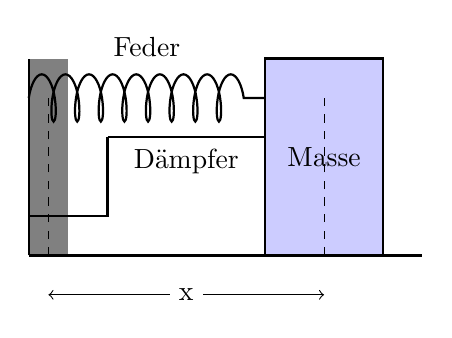
\begin{tikzpicture}
    % Draw the wall
    \fill[gray] (-1,0) rectangle (-0.5,2.5);
    \draw[thick] (-1,0) -- (-1,2.5);

    % Draw the spring
    \draw[thick,decorate,decoration={coil,aspect=0.3,segment length=3mm,amplitude=3mm}] (-1,2) -- (2,2) node[midway,above=4mm] {Feder};

    % Draw the damper
    \draw[thick] (-1,0.5) -- (0,0.5) -- (0,1.5);
    \draw[thick] (0,1.5) -- (2,1.5) node[midway,above=-6mm] {D\"ampfer};

    % Draw the mass
    \fill[blue!20!white] (2,0) rectangle (3.5,2.5);
    \draw[thick] (2,0) -- (2,2.5) -- (3.5,2.5) -- (3.5,0) -- cycle;
    \node at (2.75,1.25) {Masse};

    % Ground and vertical lines
    \draw[thick] (-1,0) -- (4,0);
    \draw[dashed] (-0.75,0) -- (-0.75,2);
    \draw[dashed] (2.75,0) -- (2.75,2);
    
    % Distance annotation
    \draw[<->] (-0.75,-0.5) -- (2.75,-0.5) node[midway,fill=white] {x};
\end{tikzpicture}
\end{center}


  \item \textbf{Elektrische Schaltkreise:} In der Elektrotechnik kann die Gleichung einen RLC-Schaltkreis (einen Schaltkreis, der einen Widerstand \( R \), eine Induktivität \( L \), und einen Kondensator \( C \) enthält) beschreiben. Hier könnte \( y(t) \) die elektrische Ladung oder den Strom darstellen, \( 2 \rho = R/L \) und \( \omega^2 = 1/(LC)\). Das Verhalten des Schaltkreises — ob er oszilliert oder schnell stabilisiert wird — hängt von den Werten dieser Komponenten ab.

\begin{center}
\begin{circuitikz}
    \draw
    % Voltage source
    (0,0) to[V, v=$V_s$, invert] (0,3)
    % Resistor
    to[R, l=$R$, v<=$V_R$] (3,3)
    % Inductor
    to[L, l=$L$, v<=$V_L$] (6,3)
    % Capacitor
    to[C, l=$C$, v<=$V_C$] (6,0)
    % Connect back to the voltage source
    -- (0,0);

    % Labels
    \node at (3,1.5) {RLC Stromkreis};
\end{circuitikz}
\end{center}
\end{enumerate}
Diese Gleichung ist allgemein bekannt als \textit{"Gedämpfter harmonischer Oszillator"} oder einfach als \textit{"Gedämpfter Oszillator"}. Sie umfasst drei spezifische Szenarien basierend auf dem Wert von \( \rho \) im Vergleich zu \( \omega \):
\begin{enumerate}
  \item \textbf{Überdämpft (\( \rho > \omega \)):} Das System kehrt ohne Oszillation langsam zum Gleichgewicht zurück.
  \item \textbf{Kritisch gedämpft (\( \rho = \omega \)):} Das System kehrt so schnell wie möglich ohne Oszillation zum Gleichgewicht zurück.
  \item \textbf{Untergedämpft (\( \rho < \omega \)):} Das System oszilliert mit einer Amplitude, die allmählich auf null abnimmt.
\end{enumerate}
\textbf{Aufgabe:}
\smallskip
Bestimmen Sie die Lösung der DGl für alle drei Fälle: überdämpft, kritisch gedämpft und untergedämpft.\\ \\
\textbf{Hinweis:} Bestimmen Sie das charakteristische Polynom und seine Nullstellen und verwenden Sie den Exponentialansatz. Man betrachte alle drei Fälle, in denen die Nullstellen einfach, doppelt oder komplex konjiugiert sind.
}


\Loesung{
Fall 1: Überdämpft (\(\rho > \omega\))
Die Wurzeln sind reell und unterschiedlich:
\[
\lambda = -\rho \pm \sqrt{\rho^2 - \omega^2}
\]
mit der Lösung:
\[
y(t) = Ae^{(-\rho + \sqrt{\rho^2 - \omega^2})t} + Be^{(-\rho - \sqrt{\rho^2 - \omega^2})t}
\]
Fall 2: Kritische Dämpfung (\(\rho = \omega\))
Die charakteristische Gleichung vereinfacht sich zu:
\[
\lambda^2 + 2\omega \lambda + \omega^2 = 0
\]
mit einer doppelten Wurzel \(\lambda = -\omega\). Die Lösung ist:
\[
y(t) = (A + Bt)e^{-\omega t}
\]
Fall 3: Untergedämpft (\(\rho < \omega\))
Die Wurzeln sind komplex:
\[
\lambda = -\rho \pm i\sqrt{\omega^2 - \rho^2}
\]
was zu der Lösung führt:
\[
y(t) = e^{-\rho t}(A \cos(\sqrt{\omega^2 - \rho^2} t) + B \sin(\sqrt{\omega^2 - \rho^2} t))
\]

}


\ErgebnisC{harmonischerOszillator}{
Fall 1: $y(t) = Ae^{(-\rho + \sqrt{\rho^2 - \omega^2})t} + Be^{(-\rho - \sqrt{\rho^2 - \omega^2})t}$,\\
Fall 2: $y(t) = (A + Bt)e^{-\omega t},$\\
Fall 3: $y(t) = e^{-\rho t}(A \cos(\sqrt{\omega^2 - \rho^2} t) + B \sin(\sqrt{\omega^2 - \rho^2} t)).$
}

